\documentclass[12pt]{article}
\author{Maedeh Karkhaneh Yousefi}
\title{HW2-3}
\usepackage{graphicx}
\usepackage{float}
\begin{document}
\maketitle
I reckon a linear model, especially linear regression is the best model to fit the data. That's because the target is continuous. 
I used MinMaxScaler and OrdinalEncoder as a preprocessing procedure.
\part{Regression}
\paragraph*{}
\textbf{Linear Regression}
\\ The linear regression score is: 0.7296646657433239 (73 percent)
\begin{figure}[H]
\centering
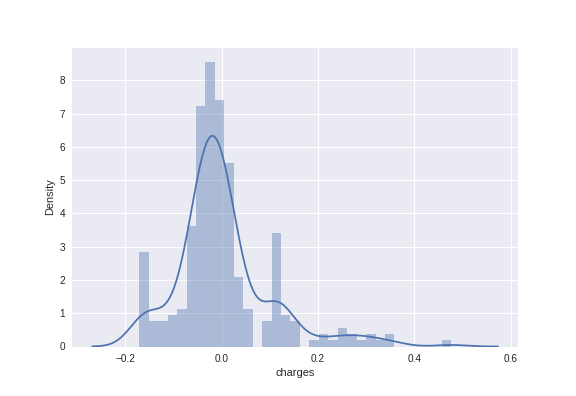
\includegraphics[width=\textwidth]{linearR (1).png}
\label{mesh:fig1}
\caption{The distplot of prediction-ytest for charges. One can see 2 other peeks, which may show 2 more classes.}
\end{figure}
\pagebreak
\textbf{Linear Regression (Polynomial Features included)}\\
The score is : 0.8199104895969911 (82 percent)
\begin{figure}[H]
\centering
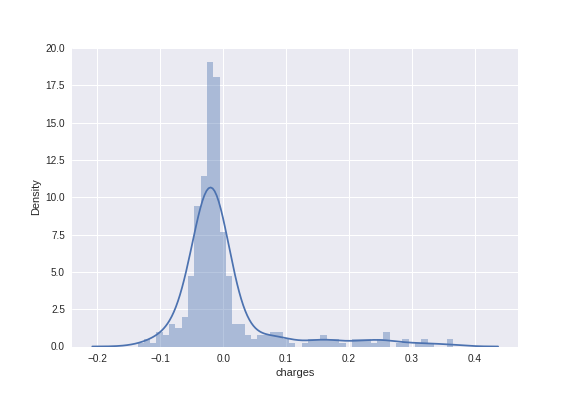
\includegraphics[width=\textwidth]{linearR_withPoly.png}
\label{mesh:fig1}
\caption{The distplot of prediction-ytest for charges. You can see that those other peaks are gone and most of the error is distributed over the range of -0.1 to 0.1. }
\end{figure}
\pagebreak
\textbf{SVR with Linear Kernel}\\
The SVR (kernel = linear) is: 0.7110971727822234 (71 percent)
\begin{figure}[H]
\centering
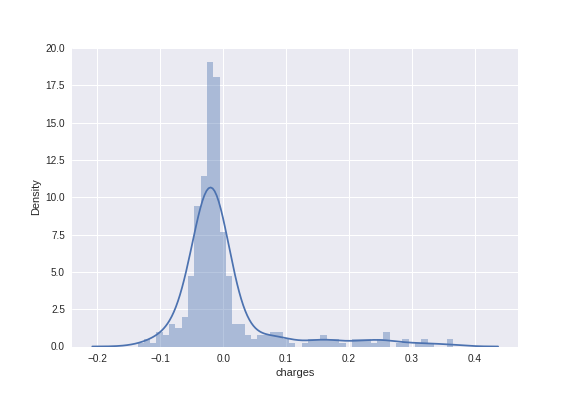
\includegraphics[width=\textwidth]{linearR_withPoly.png}
\label{mesh:fig1}
\caption{The distplot of prediction-ytest for charges. The results show a distribution of error between the range of -1 to -1, which was less for linear regression.}
\end{figure}
\pagebreak
\textbf{SVR with Poly Kernel}\\
The SVR ( kernel = poly ) score is: 0.6842361729120802 (68 percent)
\begin{figure}[H]
\centering
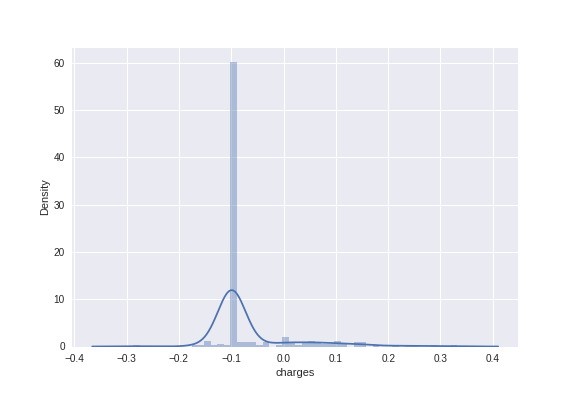
\includegraphics[width=\textwidth]{svr_poly1.png}
\label{mesh:fig1}
\caption{The distplot of prediction-ytest for charges. There is an obvious peak at -0.1, which shows that most of the data have an error of 0.1.}
\end{figure}
\pagebreak
\textbf{Random Forest Regressor}\\
The score is : 0.8262341327080196 (83 percent)
\begin{figure}[H]
\centering
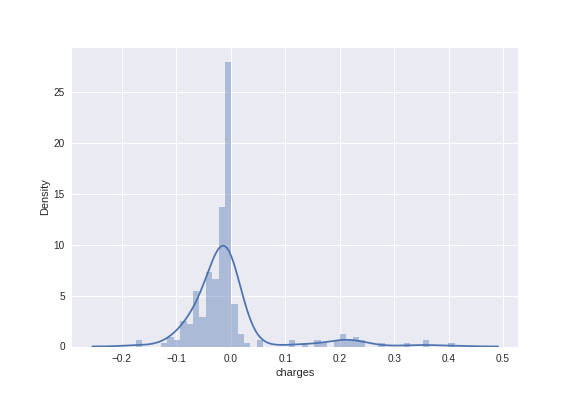
\includegraphics[width=\textwidth]{rand_forest_reg (1).png}
\label{mesh:fig1}
\caption{The distplot of prediction-ytest for charges. The errors are biased toward the left part of the plot.}
\end{figure}
\pagebreak
\textbf{PCA}
I used PCA for finding the two most important components in the models.
\begin{figure}[H]
\centering
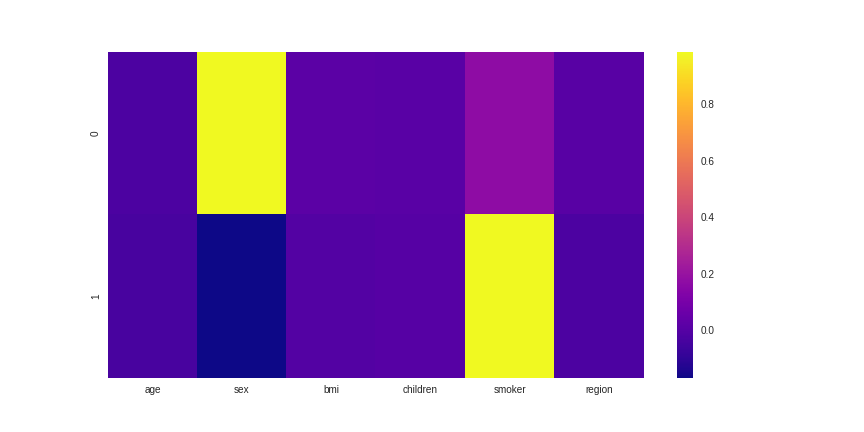
\includegraphics[width=\textwidth]{comp_heatmap.png}
\label{mesh:fig1}
\caption{From the plot one can see that smoke and sex have the most effect on those two components.}
\end{figure}
\textbf{KNN}\\
I could only use KNeighborsClassifier after classifying 'charge' into 5 classes, each representing a range of 1000 values. 
\begin{figure}[H]
\centering
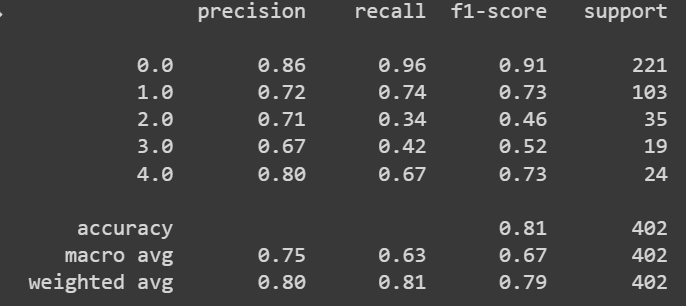
\includegraphics[width=0.5\textwidth]{KNN_report.png}
\end{figure}
The confusion matrix is:
\begin{figure}[H]
\centering
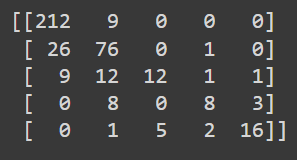
\includegraphics[width=0.3\textwidth]{matrics.png}
\end{figure}
\pagebreak
\part{Clustering}
\begin{figure}[H]
\centering
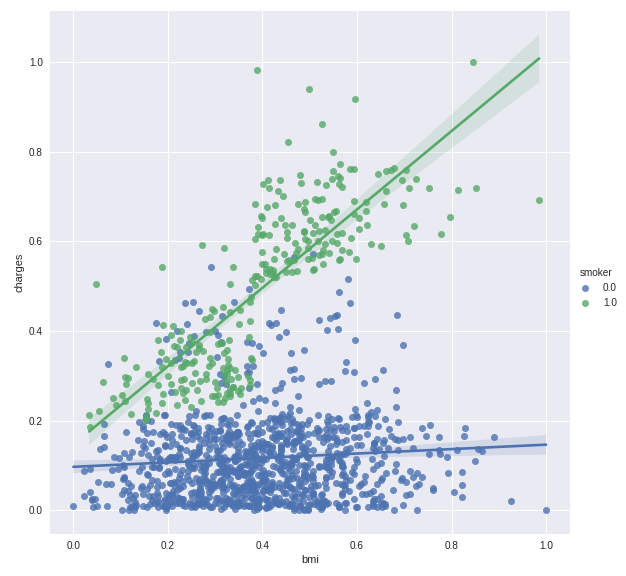
\includegraphics[width=\textwidth]{lmplot_bmi.png}
\label{mesh:fig1}
\caption{Charge-bmi lmplot with hue=smoker.}
\end{figure}
I used Kmeans for clustering, which gave me completeness score = 0.9999999999999996 and homogeneity score = 0.7772742676688331. The results are amazing actually!
\end{document}